\chapter{Activation Functions}
La maggior parte delle hidden unit consiste di una trasformazione affine $w x + b$
dell'input $x$ a cui viene applicata una funzione $g(w x + b)$ chiamata funzione di attivazione.

Le funzioni di attivazione non lineari permettono al modello di apprendere una struttura più complessa nei dati.

Solitamente si utilizza la stessa activation function in tutti gli hidden layer.

\section{Sigmoid and Hyperbolic Tangent}
Entrambe le funzioni sono differenziabili e monotoniche, mentre la loro derivata non è monotonica.

\begin{figure}
  \centering
  \begin{minipage}{0.46\linewidth}
    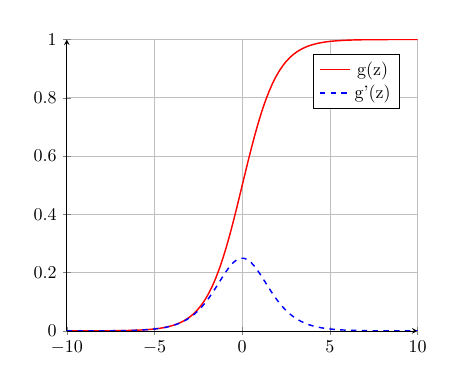
\begin{tikzpicture}[scale=0.65]
      \begin{axis}[
          axis x line = bottom,
          axis y line = left,
          grid = major,
          legend style={at={(0.95, 0.95)}},
        ]
        %\addplot[black, domain=-10:10, samples=2, forget plot] coordinates {(0,0)(0,1)};
        \addplot[thick, red, domain=-10:10, samples = 100]{1/(1+exp(-x))};
        \addplot[thick, dashed, blue, domain=-10:10, samples = 100]{(1/(1+exp(-x)))*(exp(-x)/(1+exp(-x)))};
        \addlegendentry{g(z)}
        \addlegendentry{g'(z)}
      \end{axis}
    \end{tikzpicture}
    \caption{Sigmoide}
  \end{minipage}
  \hfill
  \begin{minipage}{0.46\linewidth}
    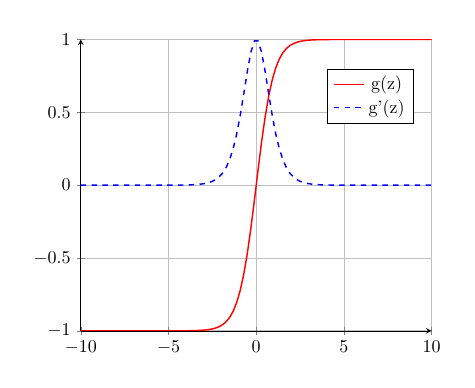
\begin{tikzpicture}[scale=0.65]
      \begin{axis}[
          axis x line = bottom,
          axis y line = left,
          grid = both,
          legend style={at={(0.95, 0.9)}},
        ]
        %\addplot[black, domain = -10:10, samples=2, forget plot] coordinates {(0,-1)(0,1)};
        \addplot[thick, red, domain = -10:10, samples = 100]{(exp(x)-exp(-x))/(exp(x)+exp(-x))};
        \addplot[thick, dashed, blue, domain = -10:10, samples = 100]{1-((exp(x)-exp(-x))/(exp(x)+exp(-x)))^2};
        \addlegendentry{g(z)}
        \addlegendentry{g'(z)}
      \end{axis}
    \end{tikzpicture}
    \caption{Tangente iperbolica}
  \end{minipage}
\end{figure}

La sigmoide è specialmente usata nell'output unit se l'output voluto è una probabilità poiché la sigmoide ha valori tra 0 e 1.

Il vantaggio della tangente iperbolica (tanh) è che i valori vengono mappati tra -1 e 1. Quindi i valori negativi in valori fortemente negativi, mentre i valori vicino a zero vengono mappati vicino a zero.

La sigmoide e la tangente iperbolica soffrono del problema della scomparsa del gradiente (vanishing gradient).
Grandi cambiamenti nell'input corrispondono a piccoli cambiamenti nell'output, rendendo di conseguenza le derivate piccole.
Durante la backpropagation le derivate vengono moltiplicate insieme, quindi al crescere del numero di layer il gradiente scomparirà sempre di più.

Entrambe le funzioni sono molto sensibili a cambiamenti vicino al punto centrale, 0.5 per tanh e 0 per la sigmoide.

\section{ReLU}
La Rectified Linear Unit (ReLU) è la funzione di attivazione più comune negli hidden layers.
E' semplice da implementare e calcolare, inoltre è meno soggetta al problema del vanishing gradient.
Tuttavia può soffrire di altri problemi come la saturazione o neuroni morti.

Non è una funzione lineare e non è differenziabile nel punto 0. Nella pratica è trascurabile poiché è poco probabile ottenere 0.
Per valori negativi il risultato sarà zero e quindi i neuroni non verranno attivati rendendo sparsa la rete e quindi più semplice da computare.

\begin{figure}[ht]
  \centering
  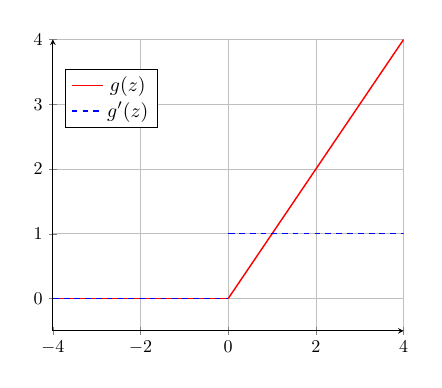
\begin{tikzpicture}[scale=0.65]
    \begin{axis}[
        axis x line = bottom,
        axis y line = left,
        grid = both,
        ymin=-0.5, ymax=4,
        xmin=-4, xmax=4,
        legend style={at={(0.3, 0.9)}, nodes={scale=1.1}},
      ]
      \addplot[thick, red, domain = -4:0, samples = 100, forget plot]{0};
      \addplot[thick, red, domain = 0:4, samples = 100]{x};
      \addplot[thick, dashed, blue, domain = 0:4, samples = 100]{1};
      \addplot[thick, dashed, blue, domain = -4:0, samples = 100]{0};
      \addlegendentry{$g(z)$}
      \addlegendentry{$g'(z)$}
    \end{axis}
  \end{tikzpicture}
  
  $g(z) = \max(0, z)$
  \caption{funzione ReLU e la sua derivata}
\end{figure}

\subsection*{Generalization of ReLU}

\textbf{Softplus}: versione smussata che approssima la ReLU e la rende derivabile in 0.
nella pratica non funziona come dovrebbe.

\begin{figure}[ht]
  \centering
  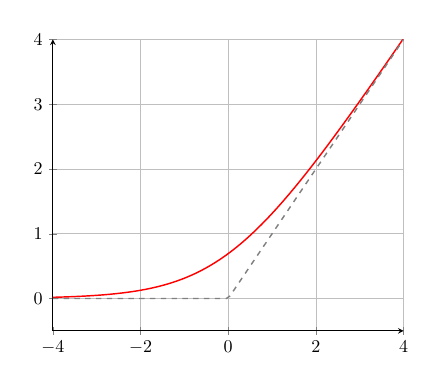
\begin{tikzpicture}[scale=0.65]
    \begin{axis}[
        axis x line = bottom,
        axis y line = left,
        grid = both,
        ymin=-0.5, ymax=4,
        xmin=-4, xmax=4,
        legend style={at={(0.6, 0.9)}, nodes={scale=1.1}},
      ]
      \addplot[thick, red, domain = -4:4, samples = 100]{ln(1 + e^x)};
      \addplot[thick, dashed, gray, domain = -4:4, samples = 100]{max(0, x)};
    \end{axis}
  \end{tikzpicture}

  $g(x) = \ln(1 + e^x)$
  \caption{Softplus}
\end{figure}

Possono essere definite altre forme di ReLU tramite la seguente formula:
\begin{align*}
  h_i = g(z, \alpha)_i = \max(0, z_i) + \alpha_i \min(0, z_i)
\end{align*}

\textbf{Absolute value rectification}: utile per trovare features che siano invarianti per qualche caratteristica. $\alpha_i = -1,\; g(z) = |z|$

\textbf{Leaky ReLU}: per valori negativi viene definita una componente lineare molto piccola con $\alpha_i = 0.01$. Può essere utile nelle reti con tanti neuroni disattivati.

\textbf{Parameter RLU}: il parametro $\alpha_i$ viene imparato dalla rete

\begin{figure}[ht]
  \centering
  \begin{minipage}{0.32\linewidth}
    \centering
    Absolute Value Rectification

    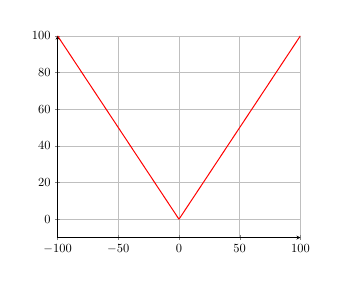
\begin{tikzpicture}[scale=0.45]
      \begin{axis}[
          axis x line = bottom,
          axis y line = left,
          grid = both,
          ymin=-10, ymax=100,
          xmin=-100, xmax=100,
          legend style={at={(0.6, 0.9)}},
        ]
        \addplot[thick, red, domain = -100:0, samples = 100, forget plot]{-x};
        \addplot[thick, red, domain = 0:100, samples = 100]{x};
      \end{axis}
    \end{tikzpicture}

    \bigskip
    $g(z) = |z|$
  \end{minipage}
  \begin{minipage}{0.32\linewidth}
    \centering
    \bigskip
    Leaky ReLU

    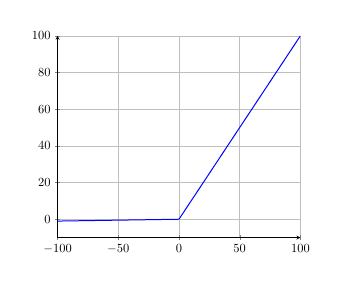
\begin{tikzpicture}[scale=0.45]
      \begin{axis}[
          axis x line = bottom,
          axis y line = left,
          grid = both,
          ymin=-10, ymax=100,
          xmin=-100, xmax=100,
          legend style={at={(0.5, 0.9)}},
        ]
        \addplot[thick, blue, domain = -100:0, samples = 100, forget plot]{0.01 * x};
        \addplot[thick, blue, domain = 0:100, samples = 100]{x};
      \end{axis}
    \end{tikzpicture}

    \bigskip
    $g(z) = \max(0, 0.01 z)$
  \end{minipage}
  \begin{minipage}{0.32\linewidth}
    \centering
    \bigskip
    Parametric ReLU

    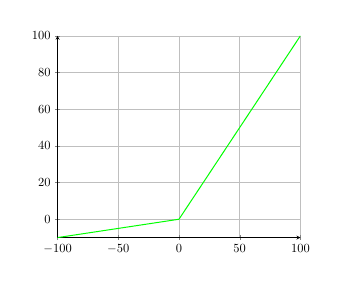
\begin{tikzpicture}[scale=0.45]
      \begin{axis}[
          axis x line = bottom,
          axis y line = left,
          grid = both,
          ymin=-10, ymax=100,
          xmin=-100, xmax=100,
          legend style={at={(0.6, 0.9)}},
        ]
        \addplot[thick, green, domain = -100:0, samples = 100, forget plot]{0.1 * x};
        \addplot[thick, green, domain = 0:100, samples = 100]{x};
      \end{axis}
    \end{tikzpicture}

    \bigskip
    $g(z) = \max(0, \alpha z)$
  \end{minipage}
\end{figure}

% fare così
% https://www.google.com/url?sa=i&url=https%3A%2F%2Fwww.researchgate.net%2Ffigure%2Fa-Sigmoid-the-logistic-function-which-has-an-S-shaped-curve-b-ReLU-rectified_fig4_311612430&psig=AOvVaw3zj0VOEvq-oCIkNhPz8CgL&ust=1636327134299000&source=images&cd=vfe&ved=0CAsQjRxqFwoTCOj5ueHvhPQCFQAAAAAdAAAAABAJ

\textbf{Maxout units}: impara la funzione da se.
Viene divisa il parametro $z$ in gruppi da $k$ parti e viene ritornato il massimo di ogni gruppo.
%
\begin{align*}
  g(z)_i = \underset{j}{\max} \; z_j \qquad j \in G^{(i)}: \text{indice j-esimo del gruppo $G^{(i)}$}
\end{align*}
%
Dato che richiede più parametri da essere imparati sono necessario più dati o più regolarizzazione.
